In order to study the collisions coming from high energy experiments, many tools have been developed. In \Sec{sec:PSmuRmuF}, the physics of hadron collision at high energies are presented. These insights are used to generate events via Monte Carlo event generators, explained in \Sec{sec:eventgeneration}. 
 Machine learning helps to differentiate between signal- and background like events. In \Sec{sec:BDT}, the multivariate technique of boosted decision trees is explained. This yields powerful discriminants for separating signal and background events and provides distributions  for template-based maximum likelihood fits. The fitting method used in the search presented in this thesis is discussed in \Sec{sec:Stat}. 
\section{Hadron collisions at high energies}
\label{sec:PSmuRmuF}
All partons can be approximated as free when there is sufficiently high momentum transfer in hadron collisions. This makes it possible to treat a hadron-hadron scattering as a single parton-parton interaction. The momentum of the parton can then be expressed as a fraction of the hadron momentum 
\begin{equation}
 \vec{p}_{\mathrm{parton}} = x \vec{p}_{\mathrm{hadron}}, 
\end{equation}
where $x$ is referred to as the Bj\"orken scaling variable. The interaction $\Pproton_{\mathrm{A}} \Pproton_{\mathrm{B}} \rightarrow \mathrm{X}$ can then be factorised in terms of partonic cross sections $\hat{\sigma}_{\mathrm{ij}\rightarrow\mathrm{X}}$~\cite{Collins:1989gx}
\begin{equation}
 \sigma_{\mathrm{p}_{\mathrm{A}}\mathrm{p}_{\mathrm{B}}\rightarrow\mathrm{X}} = \sum \limits_{\mathrm{ij}} \iint dx_1 dx_2  \: f_{\mathrm{i}}^{\mathrm{A}}(x_{\mathrm{1}},Q^2)f_{\mathrm{j}}^{\mathrm{B}}(x_{\mathrm{2}},Q^2) {d\hat{\sigma}_{\mathrm{ij}\rightarrow\mathrm{X}}}, 
 \label{eq:cross}
 \end{equation}
where i and j are the partons resolved from protons A and B. The parton density functions (PDF) are denoted as  $f_{\mathrm{i}}(x_{\mathrm{j}},Q^2)$, and $Q^2$ is the factorisation scale more commonly denoted as \muF. This factorisation scale  represents the energy at which the hadronic interaction can be expressed as a product of the partonic cross section and the process independent PDF. In \fig{fig:factoscale}, the kinematic regions in $x$ and \muF\ are shown for fixed target and collider experiments.
\begin{figure}
	\centering
	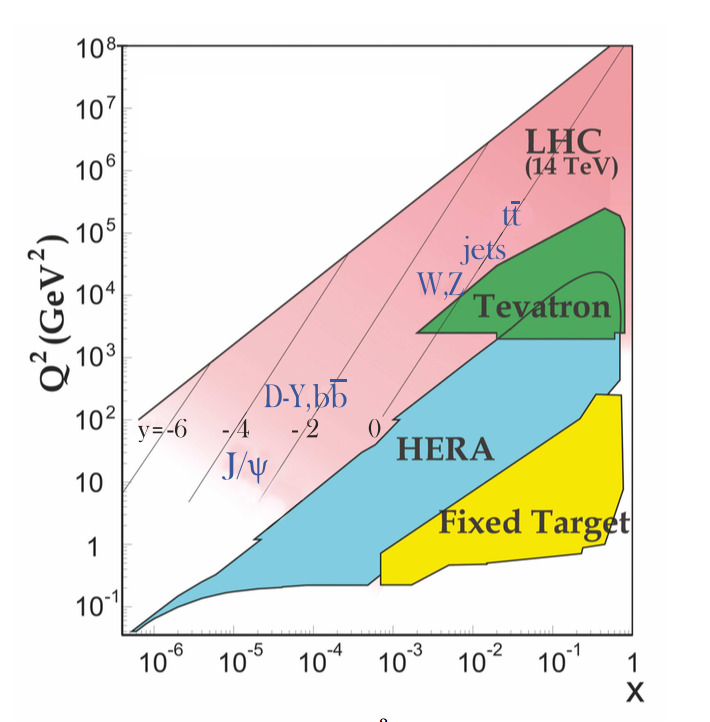
\includegraphics[width=0.5\linewidth]{3_Analysis_techniques/Figures/factoscale}
	\caption{Kinematic regions in momentum fraction $x$ and factorisation scale $Q^2$ probed by fixed-target and collider experiments. Some of the final states accessible at the LHC are indicated in the appropriate regions, where $y$ is the rapidity. In this figure, the incoming partons have $x_{1,2} = (M/14\: \TeV)e^{\pm y}$ with $Q = M$ where $M$ is the mass of the state shown in blue in the figure. For example, exclusive J$/\psi$ and $\Upsilon$ production at high $|y|$ at the LHC may probe the gluon PDF down to $x \sim  10^{-5}$. Figure taken from \cite{PDG}.}
	\label{fig:factoscale}
\end{figure}
%https://arxiv.org/pdf/1206.7024.pdf voor goede info


 The parton density functions (PDF)~\cite{Placakyte:2011az,Ball2015,Butterworth:2015oua} represent the momentum distribution of the proton amongst its partons at an energy scale \muF.  These functions are obtained from global fits to data since they can not be determined from first principles. From measurements on deep inelastic scattering using lepton-proton collision by the HERA collider~\cite{Abramowicz:1998ii}, supplemented with proton-antiproton collisions from the Tevatron~\cite{Holmes:2011ey}, and proton collision data from the ATLAS, CMS and LHCb collaborations at the LHC (Run 1)~\cite{Rojo:2015acz} the PDFs are determined and included in global PDF sets known as the \texttt{PDF4LHC} recommendation~\cite{Butterworth:2015oua}. Their measurement at scale \muF\ is extrapolated to higher energies by use of the DGLAP equations~\cite{Martin:2008cn}. Once these PDFs are known, the cross section of a certain process can be calculated and used as input for the Monte Carlo generators used to make the simulated data samples at the LHC. 
%https://amva4newphysics.wordpress.com/2016/03/10/the-inner-life-of-protons-and-artificial-neural-networks/
In the framework of this thesis,  the NLO \texttt{PDF4LHC}15\_100 set is used. This set is an envelope of three sets: \texttt{CT14}, \texttt{MMHT2014} and \texttt{NNPDF3.0}~\cite{Butterworth:2015oua}. As illustration, the dependency of the PDFs on the momentum fraction $x$ is shown for the \texttt{NNPDF3.0} set on hadronic scale $\muF^2 = 10\GeV^2$ and LHC scale $\muF^2 = 10^4\GeV^2$ in \fig{fig:nnpdf30}.  The gluon density dominated for most values of the momentum fraction, implying that it is easier to probe gluons than the quarks. When the Bj\"orken scale is to one, the parton densities of the valence quarks of the proton, up and down quarks,dominate over the gluon density. The sea quarks originating from gluon splitting, the charm, anti-up, and anti-down quarks, have lower densities in general for the proton. The resolution scale $Q^2$ is typically taken to be the energy scale of the collision. For the top quark pair production a scale of $Q^2=(350\: \GeV)^2$ is chosen, meaning that the centre-of-mass energy of the hard interaction is about twice the top quark mass.
\begin{figure}[htbp]
	\centering
	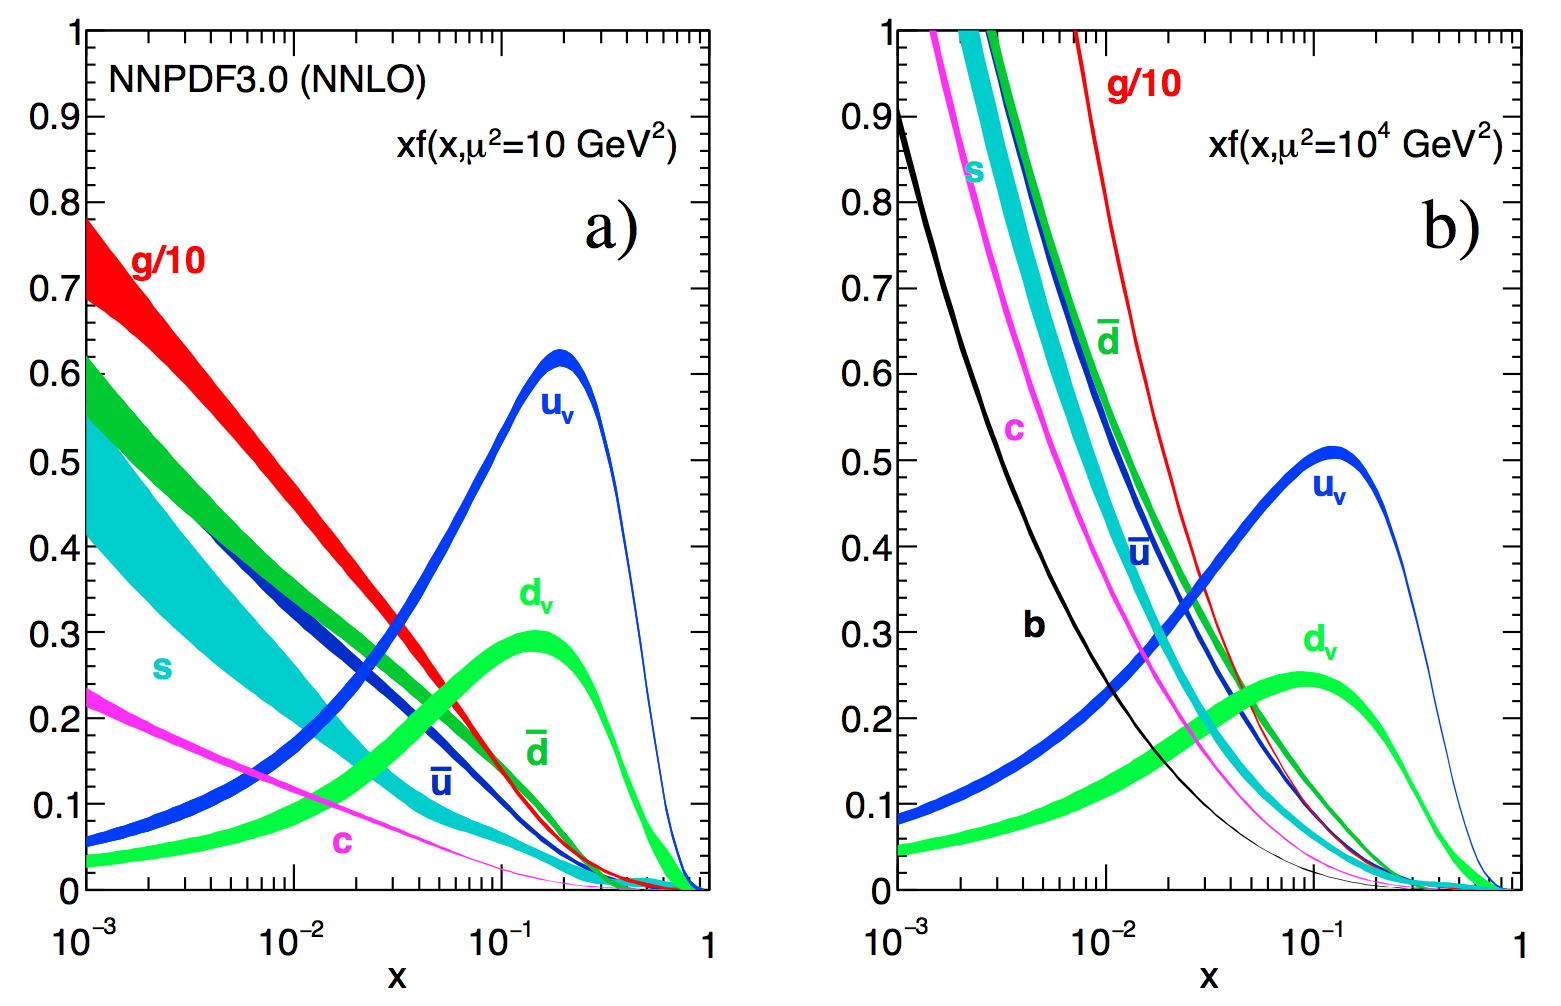
\includegraphics[width=1.\linewidth]{3_Analysis_techniques/Figures/NNPDF30}
	\caption{The momentum fraction $x$ times the parton distribution functions $f(x)$, where $f=\Pup_{\mathrm{v}}, \Pdown_{\mathrm{v}} ,\APup,\APdown,\Pstrange,\Pcharm,$ or \Pgluon\ as a function of the momentum fraction obtained in the NNLO \texttt{NNPDF3.0} global analysis at factorisation scales $\mu^2 = 10 \: \GeV^2$ (left) and $\mu^2=10^4 \: \GeV^2$ (right), with $\alpha_{\mathrm{S}}(M^2_{\PZ}) = 0.118$. The gluon PDF has been scaled down by a factor of 0.1. Figure taken from \cite{PDG}.}
	%http://pdg.lbl.gov/2017/reviews/rpp2016-rev-structure-functions.pdf
	% The higher value of the resolution scale $Q^2$, the smaller distances that are probed in the proton.
	\label{fig:nnpdf30}
\end{figure}
The uncertainty on the parton distributions is evaluated using the Hessian technique~\cite{Pumplin:2001ct}, where a matrix with a dimension identical to the number of free parameters needs to be diagonalised. In the case of \texttt{PDF4LHC}15\_100 set, this translates into 100 orthonormal eigenvectors and 200 variations of the PDF parameters in the plus and minus direction. 
%https://www.hep.ucl.ac.uk/pdf4lhc/LesHouches2016-PDF4LHC.pdf
%https://indico.cern.ch/event/525605/contributions/2152733/attachments/1267702/1877336/TOP_PAG_3_05_16_PDFs.pdf

Quantum fluctuations can cause divergences at high energies. This is solved by introducing a renormalization scale \muR\ to redefine physical quantities, making the theory still able to describe the experimental regime. A consequence of this method is that the coupling constants will run as a function of \muR. Beyond the renormalization  scale, the high energy effects such as the loop corrections to propagators (self energy) are absorbed in the physical quantities through a renormalization of the fields. In particular, the running behaviour of the strong coupling constant\footnote{The strong coupling constant is defined as $\alpha_{\mathrm{S}} = \frac{g_\mathrm{S}^2}{4\pi}$. } $\alpha_{\mathrm{S}}$ is found to be 
\begin{equation}
	\alpha_{\mathrm{S}} = \frac{\alpha_{\mathrm{S}}(\mu_0^2)}{1 + \alpha_{\mathrm{S}}(\mu_0^2) \frac{33 - 2 n_{\mathrm{f}}}{12 \pi}\mathrm{ln}\left(\frac{|\muR^2|}{\mu_0^2}\right)}, 
	\label{eq:couplingstrength}
\end{equation}
with $n_{\mathrm{f}}$ the number of quarks and $\mu_0$ the reference scale at which the coupling is known. The current world average of the strong coupling constant at the \PZ\ boson mass is $\alpha_{\mathrm{S}}(\muR = \mZ) = 0.1181 \pm 0.0011$~\cite{PDG}. From  \eq{eq:couplingstrength} one can see easily that the coupling strength decreases with increasing renormalization scale, this is known as asymptotic freedom. Additionally, following the behaviour of $\alpha_{\mathrm{S}}(\muR^2)$, a limit $\Lambda_{\mathrm{QCD}} \approx 200 \: \MeV$ is found for which $\alpha_{\mathrm{S}}$ becomes larger than one. Under this limit, the perturbative calculations of observables can no longer be done.
% Mandl and shaw pagina 352!



%The cross section $\sigma$ of scattering process with a flux\footnote{This entity is more commonly referred to as Luminosity.} $\lumi= \rho v$ of incoming particles with particle density $\rho$ and velocity $v$ is defined as the number of interactions per unit density ($\rho=1$)\footnote{The cross section is usual expressed in barn, $1b = 10^{-28}\m^2$. The number of interactions per time is given by $\frac{dN}{dt} = \lumi \sigma$}. 
Cross sections can be written in terms of interacting vertices contributing to the matrix element (ME) originating from elements of a perturbative series~\cite{Mandl:1236742}, allowing them to be expanded as a power series of the coupling constant $\alpha$ 
\begin{equation}
 \sigma  = \sigma_{\mathrm{LO}} \left(1 + \left(\frac{\alpha}{2\pi}\right)\sigma_1  + \left(\frac{\alpha}{2\pi}\right)^2\sigma_2 + ...\right).
\end{equation}
Leading order (LO) accuracy contains the minimal amount of vertices in the process, then depending on where the series is cut-off one speaks of next-to-leading order (NLO), or next-to-next-to-leading order (NNLO) accuracy in $\alpha$. Predictions including higher order corrections tend to be less affected by theoretical uncertainties originating from a variation of the chosen renormalization and factorisation scales. 
% zie thesis matthias p 21 bovenaan

\section{Event generation}
\label{sec:eventgeneration}
In order to compare reconstructed data with theoretical predictions, collision events are generated and passed through a simulation of the CMS detector and an emulation of its read-out. For the detector simulation, a so-called Full Simulation package~\cite{1742-6596-396-2-022003,1742-6596-664-7-072022}  based on the \Geant4 toolkit~\cite{AGOSTINELLI2003250} is employed. This allows detailed simulations of the interactions of the particles with the detector material. 
\subsection{Fundamentals of simulating a proton collision}
The generation of  $\Pproton\Pproton \rightarrow \mathrm{X}$ events is subdivided into sequential steps~\cite{Seymour:2013ega,Sjostrand:2009ad,Hoche:2014rga}, as shown in \fig{fig:ppcollision}.
\begin{figure}[htbp]
	\centering
	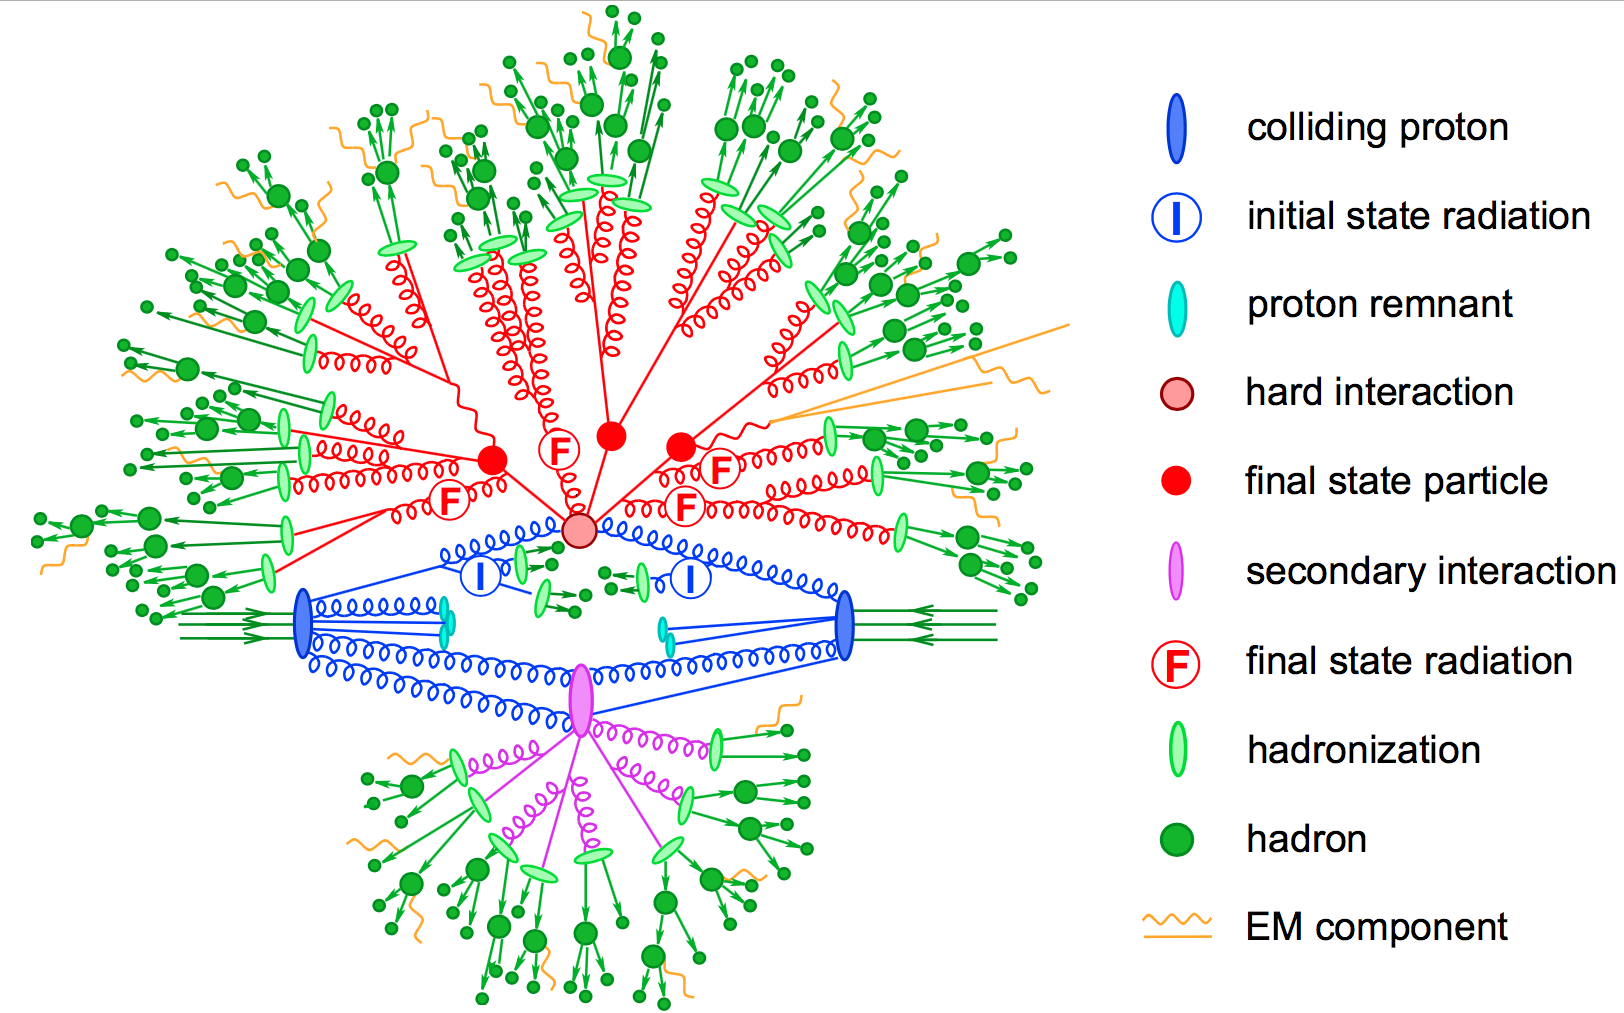
\includegraphics[width=1.\linewidth]{3_Analysis_techniques/Figures/MCeventwithlegend}
	\caption{Sketch of a hadron collision as simulated by a Monte-Carlo event generator. The red blob in the centre represents the hard collision, surrounded by a tree-like structure representing Bremsstrahlung as simulated by parton showers. The purple blob indicates a secondary hard scattering event. Parton-to-hadron transitions are represented by light green blobs, dark green blobs indicate hadron decays, while yellow lines signal soft photon radiation. Figure taken from~\cite{Hoche:2014rga}.}
	\label{fig:ppcollision}
\end{figure}

The interaction of two incoming protons is often soft and elastic leading to events that are not interesting in the framework of this thesis. More intriguing are the hard interactions between two partons from the incoming protons. The event generation starts from the matrix elements of a hard scattering process of interest. The corresponding cross section integral is sampled using Monte Carlo techniques and the resulting sample of events reflects the probability distribution of a process over its final state phase space. A parton shower (PS) program is then used to simulate the hadronisation of final state partons,  coming from the sample of events of the hard interaction, into hadrons which then decay further. On top of this,  radiation of soft gluons or quarks from initial or final state partons is simulated. These are respectively referred to as initial state radiation (ISR) or final state radiation (FSR). The contributions from soft secondary interactions, the so-called underlying event (UE), and colour reconnection effects are also taken into account. 
A brief overview of the programs used for the event generation of the signal and main background processes used in the search presented in this thesis,  is given in \Sec{sec:programs}.

\subsection{Programs for event generation}
\label{sec:programs}
The \texttt{FEYNRULES} package~\cite{Alloul:2013bka} allows for the calculation of  the Feynman rules in momentum space for any quantum field theory model. By use of a Lagrangian, the set of Feynman rules associated with this Lagrangian is calculated. Via the \UFO\ (UFO)~\cite{Degrande:2011ua} the results are then passed to matrix element generators. 


The \MG\  program~\cite{Alwall:2011uj} is used to interpret the physics model and calculate the corresponding Feynman diagrams and matrix elements. After this, \ME~\cite{Mangano:2006rw} is used to calculate the corresponding partons. These generated parton configurations are then merged with \Pythia~\cite{Sjostrand2015159,Sjostrand:2006za,Sjostrand:2014zea} parton showers using the MLM merging scheme~\cite{Alwall:2007fs}. 

The \aMCMG\ program~\cite{Alwall:2014hca} combines the LO \MG~\cite{Alwall:2011uj} and the \aMC\ program into a common framework. This combination supports the generation of samples at LO or NLO together with a dedicated matching to parton showers  using the MC@NLO~\cite{Frixione:2002ik} or FxFx~\cite{Frederix:2012ps} schemes respectively. The FXFX scheme produces a certain fraction of events with negative weights originating from the subtraction of amplitudes that contain additional emissions from the NLO matrix element to prevent double-counting.
%or MC$@$NLO~\cite{Frederix:2012ps}  \todo{MC$@$NLO voor ME generator }



The \Powheg\ box (versions 1 and 2)~\cite{Alioli2010,1126-6708-2009-09-111,1126-6708-2007-11-070,Alioli:2010xd,Frixione:2007vw,Nason:2004rx} contains predefined implementations of various processes at NLO. It applies the \Powheg\ method for ME- to PS- matching, where the hardest radiation generated from the ME has priority over subsequent PS emission to remove the overlap with the PS simulation.

The \JHU\ generator (version 7.02)~\cite{Gritsan:2016hjl,Anderson:2013afp,Bolognesi:2012mm,Gao:2010qx} is used to generate the parton level information including full spin and polarization correlations. It is commonly used for studying the spin and parity properties of new resonances such as $\mathrm{ab}\rightarrow\mathrm{X}\rightarrow \mathrm{VV}$, where $\mathrm{V} = \PZ, \PW, \Pphoton$. 

The generation of events from processes involving the production and decay of resonances creates a computational heavy load, especially at NLO. The narrow width approximation assumes that the resonant particle is on-shell. This factorizes the production and decay amplitude, allowing to perform the simulation of the production and decay of heavy resonances like top quarks or Higgs bosons to be performed in separate steps. The \MS\ program~\cite{Artoisenet:2012st} extends this approach and accounts for off-shell effects through a partial reweighting of the events. Additionally, spin correlation effects between production and decay products are taken into account. 

The \Pythia\ program (versions 6 and 8)~\cite{Sjostrand2015159,Sjostrand:2006za,Sjostrand:2014zea} generates events of various processes at LO. However, more commonly it is only used for its PS simulation and is then  used after other LO and NLO event generators to perform subsequent parton showering, hadronisation, and simulation of the underlying event.  In this thesis the underlying event tunes~\cite{Khachatryan2016}  are the CUETP8M2T4, CUETP8M1 and CUETP8M2. 





The detector response is simulated via the \Geant 4~\cite{AGOSTINELLI2003250} program. This program tracks the particles through the detector material via a detailed description of the detector and generates several hits throughout several sensitive layers. 
In addition, the response of the detector electronics to these hits are simulated. 


\subsection{Generating FCNC top-Z interactions}
The FCNC processes are generated by interfacing the Lagrangian in \eq{eq:EFTlag} with \aMCMG\ by means of the \FR\ package and its  \UFO\ format.  The complex chiral parameters are arbitrary chosen to be $f^{\mathrm{L}}_{\mathrm{X}\Pquark} = 0$ \todo{RH and LH gave the same resulting variables and RH is easier to simulate since those are singlets under SU2 (no doublet with b)} and  $f^{\mathrm{R}}_{\mathrm{X}\Pquark} = 1$. The processes are generated with the \aMCMG\ (version 2.2.2) and showered with \Pythia\ (version 8.22). The signal consists of two components: events describing the top quark pair production followed by an FCNC decay of one top quark ($\Ptop\rightarrow\PZ \Pquark$), and events with the FCNC single top quark production ($\PZ\Pquark\rightarrow\Ptop$) for which the top quark decays according to the\SM. The leading order generation of the single top quark FCNC process \tZ+0,1 jet including a merging technique can not be done since \tZ+1 jet also contains contributions from top quark pair FCNC where one quark is decaying in \tZ. Therefore, single top quark and top quark pair processes are generated independently, where the single top quark process is generated without the extra hard jet, and the top quark pair FCNC process is generated with up to two extra jets.


 The signal rates are estimated by use of the \aMCMG\ program for estimating the partial widths. The anomalous couplings are left free to float for this estimation, and only one coupling is allowed to be non-vanishing at a time. The results are presented in \tab{tab:partialwidths}.
\begin{table}[htbp]
	\centering
	\caption{Leading order partial widths related to the anomalous decay modes of the top quark, where the new physics scale $\Lambda$ is given in \GeV.}
	\begin{tabular}{ccrl}
		\toprule
		Anomalous coupling & vertex & \multicolumn{2}{c}{Partial decay width  (\GeV) }\\ 
		\midrule
%		\multirow{2}{*}{\kgqtl} & \Ptop\Pgluon\Pup      &  3.67 $\times 10^{5}$   & $\times\left( \kappa_{\Ptop\Pgluon\Pup} / \Lambda \right)^2$ \\
%		                    & \Ptop\Pgluon\Pcharm       &  3.66 $\times 10^{5}$   & $\times\left( \kappa_{\Ptop\Pgluon\Pcharm} / \Lambda \right)^2$ \\
%	    \multirow{2}{*}{\kfqtl} & \Ptop\Pphoton\Pup     &  1.99 $\times 10^{4}$   & $\times\left( \kappa_{\Ptop\Pphoton\Pup} / \Lambda \right)^2$ \\
%		                    & \Ptop\Pphoton\Pcharm      &  1.99 $\times 10^{4}$   & $\times\left( \kappa_{\Ptop\Pphoton\Pcharm} / \Lambda \right)^2$    \\
		\multirow{2}{*}{\kZqtl} & \Ptop\PZ\Pup          &  1.64 $\times 10^4$     & $\times\left( \kappa_{\Ptop\PZ\Pup} / \Lambda \right)^2$     \\
		                    & \Ptop\PZ\Pcharm           &   1.64 $\times 10^4$    & $\times\left( \kappa_{\Ptop\PZ\Pcharm} / \Lambda \right)^2$  \\
	\hdashline
		\multirow{2}{*}{\zZqt} & \Ptop\PZ\Pup           &   1.69 $\times 10^{-1}$ & $\times\left( \zeta_{\Ptop\PZ\Pup}  \right)^2$ \\
		                    & \Ptop\PZ\Pcharm           &   1.68 $\times 10^{-1}$ & $\times\left( \zeta_{\Ptop\PZ\Pcharm} \right)^2$ \\
%	    \multirow{2}{*}{\eHqt} & \Ptop\PHiggs\Pup       &   1.90 $\times 10^{-1}$ & $\times\left( \eta_{\Ptop\PHiggs\Pup}  \right)^2$  \\
%		                    & \Ptop\PHiggs\Pcharm       &   1.90 $\times 10^{-1}$ & $\times\left( \eta_{\Ptop\PHiggs\Pcharm}  \right)^2$ \\
			\bottomrule
	\end{tabular} 
	\label{tab:partialwidths}
\end{table}

The anomalous single top quark cross sections are calculated by convolution of the hard scattering matrix elements with the LO order set of \texttt{NN23LO1}~\cite{Ball:2012cx} % \CTEQ 6 for pheno~\cite{Pumplin:2002vw}
partons densities. The NLO effects are modelled by multiplying each LO cross section by a global $k$-factor. The LO single top quark production cross section and the global $k$-factors for the top-\PZ\ production are shown in \tab{tab:STx}. The hard scattering events are then matched to parton showers to \Pythia\ to account for the simulation of the QCD environment relevant for hadronic collisions. 
\begin{table}[htbp]
	\centering
	\caption{Leading order single top quark production cross section at a centre-of-mass of 13 \TeV\ for $\Pproton\Pproton \rightarrow \tZ$ or $\tbarZ$, where the new physics scale is given in \GeV. The NLO $k-$factors~\cite{Zhang:2011gh} are given in the last column.}
	\begin{tabular}{ccrlcc}
		\toprule
	   Anomalous  & vertex & \multicolumn{2}{c}{Cross section (\pb)} &  $\sigma_{\Pproton\Pproton\rightarrow\APtop}/\sigma_{\Pproton\Pproton\rightarrow\Ptop}$ &  NLO $k-$factor \\ 
	     coupling & & \multicolumn{2}{c}{$\Pproton\Pproton\rightarrow\Ptop + \Pproton\Pproton\rightarrow\APtop$} &   &  \\ 
		\midrule
%	   $\kappa_{\Ptop\Pgluon\Pup} / \Lambda $     &  1.29 $\times 10^{12}$  & $\times\left( \kappa_{\Ptop\Pgluon\Pup} / \Lambda \right)^2$ & 0.17 &1.50 \\
%	   $\kappa_{\Ptop\Pgluon\Pcharm} / \Lambda $  & 2.47 $\times 10^{11}$  & $\times\left( \kappa_{\Ptop\Pgluon\Pcharm} / \Lambda \right)^2$ & 0.51 &1.50 \\
%	  $\kappa_{\Ptop\Pphoton\Pup} / \Lambda $    &  1.62 $\times 10^7$  & $\times\left( \kappa_{\Ptop\Pphoton\Pup} / \Lambda \right)^2$ & 0.13 &1.40 \\
%	   $\kappa_{\Ptop\Pphoton\Pcharm} / \Lambda $ & 2.37 $\times 10^6$  & $\times\left( \kappa_{\Ptop\Pphoton\Pcharm} / \Lambda \right)^2$ & 0.50 &1.40 \\
%	   $\eta_{\Ptop\PHiggs\Pup} / \Lambda $         &  8.27 $\times 10$  & $\times\left( \kappa_{\Ptop\PZ\Pup} / \Lambda \right)^2$ & 0.13 &1.50 \\
%	   $\eta_{\Ptop\PHiggs\Pcharm} / \Lambda $      &  1.18 $\times 10$   & $\times\left( \kappa_{\Ptop\PZ\Pcharm} / \Lambda \right)^2$ & 0.50 &1.80 \\
	   \multirow{2}{*}{\kZqtl} & $\Ptop\PZ\Pup$         &  1.92 $\times 10^7$  & $\times\left( \kappa_{\Ptop\PZ\Pup} / \Lambda \right)^2$ & 0.12 &1.40 \\
	   &  $\Ptop\PZ\Pcharm $      &  2.65 $\times 10^6$  & $\times\left( \kappa_{\Ptop\PZ\Pcharm} / \Lambda \right)^2$ & 0.50&1.40 \\
	   \hdashline
	   \multirow{2}{*}{\zZqt} &$\Ptop\PZ\Pup$                    & 8.24 $\times 10$  & $\times\left( \zeta_{\Ptop\PZ\Pup} \right)^2$ & 0.14  &1.40 \\
	   &$\Ptop\PZ\Pcharm $                 &  1.29 $\times 10$  & $\times\left( \zeta_{\Ptop\PZ\Pcharm}  \right)^2$ & 0.50 & 1.40 \\
       \bottomrule
	\end{tabular} 
	\label{tab:STx}
\end{table}
\newpage
The top quark pair cross sections are derived from the \SM\ \ttbar\ cross section, calculated with \aMCMG\ at NLO at a centre-of-mass of 13 \TeV\ ($\sigma_{\ttbar}^{\mathrm{SM,NLO}} = 6.741 \times 10^{2} \pb$), and considering the decay $\ttbar \rightarrow (\Pbottom \PWpm)(\mathrm{X}\Pquark\Ptop)$. The branching fraction $\BR(\Ptop \rightarrow \Pbottom\PWpm)$ is assumed to be equal to one and the FCNC branching fraction is calculated as 
\begin{equation}
 \BR(\Ptop \rightarrow \Pquark\mathrm{X}) = \frac{ \Gamma_{\Ptop \rightarrow \Pquark\mathrm{X}} }{\Gamma_{\Ptop}^{\mathrm{SM}} + \Gamma_{\Ptop}^{\mathrm{FCNC}} }
 		\approx  \frac{ \Gamma_{\Ptop \rightarrow \Pquark\mathrm{X}} }{\Gamma_{\Ptop}^{\mathrm{SM}}} , 
\end{equation}
where $\Gamma_{\Ptop \rightarrow \Pquark\mathrm{X}}$ is given in \tab{tab:partialwidths}, $\Gamma_{\Ptop}^{\mathrm{SM}}=1.32 \GeV$~\cite{Gao:2012ja}, and the assumption $ \Gamma_{\Ptop}^{\mathrm{FCNC}} \ll \Gamma_{\Ptop}^{\mathrm{SM}}$ is made. In \tab{tab:TTx}  the resulting NLO cross sections for the top-Z FCNC interactions are given.  
\begin{table}[htbp]
	\centering
	\caption{ Next to leading order top quark pair cross section for the top-Z FCNC interactions  $\ttbar \rightarrow (\Pbottom \PWpm)(\mathrm{X}\Pquark\Ptop)$ with with a full leptonic decay at a centre-of-mass of 13 \TeV, where $\sigma_{\Pproton\Pproton\rightarrow \ttbar}^{\mathrm{SM,NLO}} = 6.741 \times 10^2 \pb$, $\BR(\PZ\rightarrow \Plepton\APlepton) = 3.36\times 3 \times 10^{-2}$, and $\BR(\PW\rightarrow \Plepton\Pnu) = 10.80\times 3 \times 10^{-2}$.}
	\begin{tabular}{cccrl}
		\toprule
		Anomalous coupling & vertex & Process &   \multicolumn{2}{c}{Cross section (\pb)}  \\ 
		\midrule
 \multirow{4}{*}{\kZqtl} &\multirow{2}{*}{$\Ptop\PZ\Pup$} & $\ttbar \rightarrow (\Pbottom \Pleptonplus\Pneutrino) (\APup \Pleptonplus \Pleptonminus)$ & 2.727 $\times 10^5$  & $\times\left( \kappa_{\Ptop\PZ\Pup}/\Lambda \right)^2$ \\
 & & $\ttbar \rightarrow (\APbottom \Pleptonminus\APneutrino) (\Pup \Pleptonplus \Pleptonminus)$ & 2.727$\times 10^5$  & $\times\left( \kappa_{\Ptop\PZ\Pup}/\Lambda \right)^2$ \\
 &\multirow{2}{*}{$\Ptop\PZ\Pcharm$} & $\ttbar \rightarrow (\Pbottom \Pleptonplus\Pneutrino) (\APcharm \Pleptonplus \Pleptonminus)$ &2.726$\times 10^5$  & $\times\left( \kappa_{\Ptop\PZ\Pcharm}/\Lambda \right)^2$ \\
& & $\ttbar \rightarrow (\APbottom \Pleptonminus\APneutrino) (\Pcharm \Pleptonplus \Pleptonminus)$ & 2.726$\times 10^5$  & $\times\left( \kappa_{\Ptop\PZ\Pcharm}/\Lambda \right)^2$ \\
\hdashline
 \multirow{4}{*}{\zZqt} & \multirow{2}{*}{$\Ptop\PZ\Pup$} & $\ttbar \rightarrow (\Pbottom \Pleptonplus\Pneutrino) (\APup \Pleptonplus \Pleptonminus)$ & 2.807   & $\times\left( \zeta_{\Ptop\PZ\Pup}\right)^2$ \\
& & $\ttbar \rightarrow (\APbottom \Pleptonminus\APneutrino) (\Pup \Pleptonplus \Pleptonminus)$ & 2.807   & $\times\left( \zeta_{\Ptop\PZ\Pup}\right)^2$ \\
&\multirow{2}{*}{$\Ptop\PZ\Pcharm$} & $\ttbar \rightarrow (\Pbottom \Pleptonplus\Pneutrino) (\APcharm \Pleptonplus \Pleptonminus)$ & 2.807  & $\times\left( \zeta_{\Ptop\PZ\Pcharm}\right)^2$ \\
& & $\ttbar \rightarrow (\APbottom \Pleptonminus\APneutrino) (\Pcharm \Pleptonplus \Pleptonminus)$ & 2.807  & $\times\left( \zeta_{\Ptop\PZ\Pcharm}\right)^2$ \\
		\bottomrule
	\end{tabular} 
	\label{tab:TTx}
\end{table}


\newpage
\subsection{Generating \SM\  background events}

The SM \tZq\ sample is generated using the \aMCMG\ generator~(version 2.2.2)~\cite{Alwall:1699128} at leading order accuracy. The \ttZ\ and triboson samples were generated using the \\\aMCMG\ generator~(version 2.2.2), interfaced through the dedicated MC${@}$NLO matching scheme~\cite{Frixione:2002ik}. The \WZ+jets and \ttW\ samples are produced with up to one additional parton at next-to-leading order accuracy using \aMCMG~(version 2.2.2) and using FxFx approach~\cite{Frederix:1481985} for matching and merging. The samples of \ttH, \WW, \ZZ,  and single top quark  production channels are generated with the \Powheg\ box (versions 1 and 2)~\cite{Alioli2010,1126-6708-2009-09-111,1126-6708-2007-11-070,Alioli:2010xd,Frixione:2007vw,Nason:2004rx}. The \JHU\ generator~\cite{Gritsan:2016hjl,Anderson:2013afp,Bolognesi:2012mm,Gao:2010qx} is used for the \tqH\ sample, while the \tWZ\ sample is generated using \aMCMG\ at leading order~\cite{Alwall:2011uj}. All events are interfaced to \Pythia~version 8.22~\cite{Sjostrand:2014zea} to simulate parton shower, hadronisation, and underlying event. Additionally, \MS\ is used for the \tZq, \WZ+jets, \ttZ, \ttW, \tWZ, and triboson samples.



The complete list of \SM\ samples is given in Table \ref{tab:samples}, along with their cross sections at a centre-of-mass of 13 \TeV. The cross sections without a reference are coming from the generator with which the sample has been made, for some of them the uncertainties are provided by the Generator Group~\cite{generator}. For each MC sample, the integrated luminosity that the sample represents is estimated as the number of simulated events divided by the cross section of the generated process. This luminosity is then matched to integrated luminosity of 35.9 \fbinv\ represented by the data used for analysis.  For processes generated with \aMCMG, the effective number of simulated events is used, taking into account positive and negative event weights. %The correction factor for those events is defined as
%\begin{equation}
%\mathrm{C} = \frac{\textnormal{Nb. of pos. weights} + \textnormal{Nb. of neg. weights}}{\textnormal{Nb. of pos. weights} - \textnormal{Nb. of neg. weights}} \times \textnormal{MC baseweight}
%\end{equation}
In \fig{fig:sigmanewv0}, a summary is given of the \SM\ cross section measurements performed by the CMS collaboration. These cross sections are all in agreement with their \SM\ predictions. 

\begin{landscape}
	\begin{table}
		\centering
		\caption{SM MC samples used in this analysis with their corresponding cross section at a centre-of-mass of 13 \TeV\ and \aMCMG\ correction C  when applicable. The generators used for each sample are indicated and the simulation of the parton shower, hadronisation, and underlying event is done by \Pythia~version 8.22~\cite{Sjostrand:2014zea} for all samples. }
		\begin{tabular}{lllll}
			\toprule
			Process & Generator & Cross section (\pb) & C  & Ref. \\ 
			\midrule
			$\WZ \rightarrow 3\Plepton\Pneutrino$ & \aMCMG+\MS& 5.26   & 1.61 & \cite{generator} \\ 
			
			\tZq\ with $\PZ\rightarrow \Pleptonplus \Pleptonminus$ & \aMCMG+\MS & 0.0758  & 3.77 & \cite{generator} \\ 
			
			\tqH\ with $\PHiggs \rightarrow \ZZ \rightarrow \Pleptonplus \Pleptonminus \Pleptonplus \Pleptonminus$& \JHU&8.80 10$^{-6}$ & - & \cite{generator}  \\ 
			
			\ttW+jets with $\PW\rightarrow \Plepton\Pneutrino$ & \aMCMG+\MS & 0.2043 $\pm$ 0.0020  &1.94 &\cite{generator} \\ 
			
			
			%/TTWJetsToQQ\_TuneCUETP8M1\_13TeV-amcatnloFXFX-madspin-pythia8/ & 0.4062$\pm$ 0.0021 & -1 \\ 
			 
			$\ttZ\rightarrow 2\Plepton+2\Pneutrino+\mathrm{other}$, with $m_{\Plepton\Plepton}>10 \;\GeV$ & \aMCMG +\MS & 0.2529 $\pm$ 0.0004 & 2.15 & \cite{generator} \\ 
			
			\ttH,no \bbbar\ decays &\Powheg& 0.2151  & - &\cite{generator} \\ 
		
			\ttH, \bbbar\ decays& \Powheg& 0.2934  & - & \cite{generator} \\ 
			 
			$\WW\rightarrow 2\Plepton2\Pneutrino$& \Powheg & 12.178  & - &\cite{Gehrmann:2014fva} \\
			
			$\ZZ\rightarrow 4\Plepton$ & \Powheg & 0.3366 & - &  \cite{generator}\\ 
			 
			\WZZ & \aMCMG+ \MS&0.05565  & 1.14 &  \cite{generator}\\ 
		
			\ZZZ  & \aMCMG&0.01398  & 1.17 &  \cite{generator}\\ 
		 
			\st\ \tWZ, with $\PZ_{\mu}\rightarrow \Pleptonplus\Pleptonminus$ & \aMCMG(LO)+\MS&0.001123 & - &  \cite{generator}\\ 
			
			%/ST\_s-channel\_4f\_leptonDecays\_13TeV-amcatnlo-pythia8\_TuneCUETP8M1 & 3 $\times$ 3.36 $^{+0.13}_{-0.12}$  & -1 \\ 
		
			\st\ t-channel \APtop  & \Powheg +\MS& 44.33 $^{+1.76}_{-1.49}$  & - &  \cite{generator} \\ 
		
			\st\ t-channel \Ptop & \Powheg +\MS & 26.38 $^{+1.32}_{-1.18}$   & - & \cite{generator} \\ 
			
			\st\  $\bar{\mathrm{t}}\PW$ & \Powheg& 35.85 $\pm$ 0.90 (scale) $\pm$ 1.70 (PDF)   & - &  \cite{generator} \\ 
		
			\st\ $\mathrm{t}\PW$ & \Powheg&35.85  $\pm$ 0.90 (scale) $\pm$ 1.70 (PDF) & - &  \cite{generator} \\ 
			
			\ttbar &\Powheg & 831.76 $^{+19.77}_{-29.20}$$^{+35.06}_{-35.06}$   & -&  \cite{generator} \\ 
			
			\DY, with $m_{\Plepton\Plepton}> \;50 \GeV$  & \aMCMG  &3 $\times$( 1921.8 $\pm$  0.6 $\pm$ 33.2 ) & 1.49 &  \cite{generator} \\ 
			
			\DY, with $10\; \GeV <m_{\Plepton\Plepton} < 50\; \GeV$ & \MG  & 18610  & - &  \cite{generator}\\ 
			\bottomrule 
		\end{tabular} 
		\label{tab:samples}
	\end{table}
\end{landscape}

\begin{figure}[htbp]
	\centering
	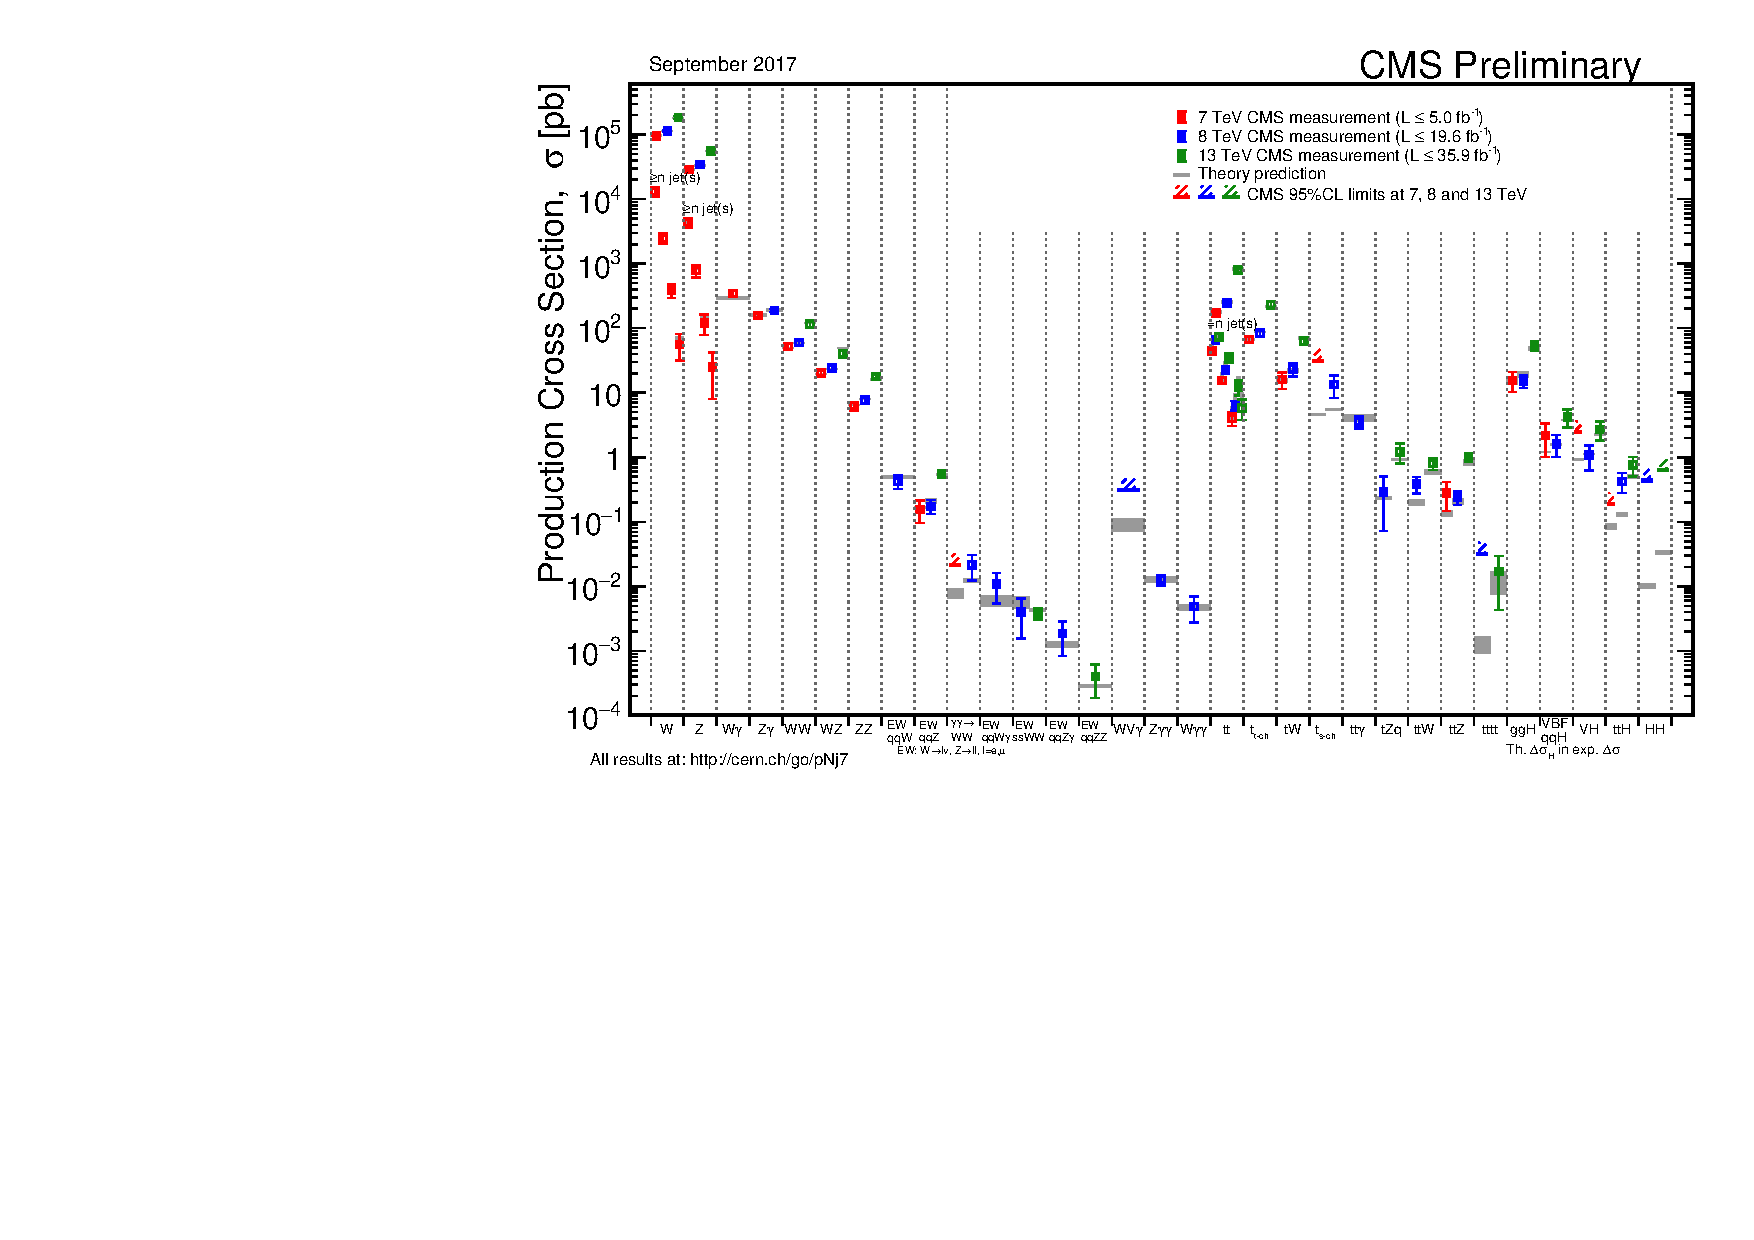
\includegraphics[width=1.\linewidth]{1_Introduction/Figures/SigmaNew_v0}
	\caption{Summary of the \SM\ cross section measurements performed by the CMS collaboration. Figure taken from \cite{summarywiki}}.
	\label{fig:sigmanewv0}
\end{figure}

%\subsection{Parton distribution functions and the hard interaction}
%\subsection{Parton showering}
%\subsection{Hadronisation and decay}
%explanation of jets https://profmattstrassler.com/articles-and-posts/particle-physics-basics/the-known-apparently-elementary-particles/jets-the-manifestation-of-quarks-and-gluons/
%\subsection{Underlying event}
\begin{comment}
%The draft document may be found at this URL: http://cds.cern.ch/record/2261310
%It is version no. 1 entitled:
%`Measurement of the underlying event using inclusive Z boson production in proton-proton collisions at sqrt(s) = 13 TeV`
% http://cms.cern.ch/iCMS/analysisadmin/cadi?ancode=FSQ-16-008
\end{comment}
%\subsection{Event reconstruction and identification}
% ICHEP https://cds.cern.ch/record/2005743
%\section{Event reconstruction}
\section{Multivariate analysis techniques: Boosted Decision Trees}
\label{sec:BDT}
The need of processing large quantities of data and discriminating between events with largely similar experimental signatures makes multivariate  analysis (MVA) a largely used method in the physics community. Multivariate classification methods based on machine learning techniques are a fundamental ingredient to most analyses. The advantage of using a MVA classifier is that it can achieve a better discrimination power with respect to a simpler analysis based on individual selection criteria or poorly discriminating variables. A risk of using MVA classifiers is overtraining.  This happens when there are too many model parameters of an algorithm adjusted to too few data points. This leads to an increase in the classification performance over the objectively achievable one.

There are many software tools that exist for MVA. In this thesis the \texttt{Tool for Multivariate Analysis} (TMVA) \cite{2007physics3039H} is used. This software is an open source project included into \texttt{ROOT}~\cite{Brun:1997pa}. 
%http://idefix.mi.infn.it/~palombo/didattica/AnalisiStatistica/mvaLectures.pdf
%All multivariate techniques in TMVA belong to supervised learning algorithms.
 By training on events for which the classification is known, a mapping function is determined that describes a classification or an approximation of the underlying behaviour defining the target value (regression). In this thesis boosted decision trees (BDT) are employed for the classification of events as implemented in the \texttt{TMVA} framework~\cite{2007physics3039H}. This multivariate technique is based on a set of decision trees where each tree yields a binary output depending on the fact that an event is signal- or background-like. This has as advantage  that several discriminating variables can be combined into a powerful one-dimensional discriminant D. 

The decision tree is constructed by training on a dataset for which the outcome is already provided, such as simulation datasets with signal and background processes (supervised learning). Different trees can be combined into a forest where the final output is determined by the majority vote of all trees, so-called boosting. This stabilises the decision trees against statistical fluctuations and makes it possible to keep the decision trees very shallow, making the method more robust against overtraining. Examples of such boosting algorithms are Adaptive Boosting (AdaBoost) and Gradient Boosting~\cite{2014arXiv1403.1452M}.  In this thesis Gradient boost is used with a learning rate of 0.2-0.3 and the depth of the tree is set to three. Additionally, the Gradient boost is used in combination with bagging, so-called stochastic gradient boosting. Bagging smears the statistical fluctuations in the training data and therefore  stabilises the response of the classifier and increases the performance by eliminating overtraining.  More information about stochastic gradient boosting can be found in Ref.~\cite{Behnke:2013:DAH:2564838}.% In stochastic gradient boosting the bagging resampling procedure uses random sub-samples of the training events for growing the trees.

%In \fig{fig:BDTexample} a schematic view of de decision tree is shown. The starting point is the root node. Then a consecutive set of a total of $i$ questions (nodes) regarding discriminating variables $x_\mathrm{i}$ are asked with only two possible answers per question (binary splits). The decision tree is constructed by training on a dataset for which the outcome is already provided, such as simulation datasets with signal and background processes (supervised learning). For each node a criterion $x_{\mathrm{i}}>C_{\mathrm{i}}$ is found by maximizing the separation gain between nodes 
%\begin{equation}
%\mathrm{separation}\:\mathrm{gain} \approx \mathrm{gain(parent)} - \mathrm{gain (daughter,Signal)} - \mathrm{gain (daughter,Background)},
%\end{equation}
%with the gain computed using the Gini index
%\begin{equation}
% \mathrm{gain(cell)} \approx p (1-p), 
%\end{equation}
%where $p$ denotes the purity of a selection $x>C$. This is repeated until the maximum of nodes is reached and at the end of the sequence, the leaf nodes are labelled either signal S or background B, depending on the majority of events that end up on those nodes. 
%\begin{figure}[htbp]
%	\centering
%	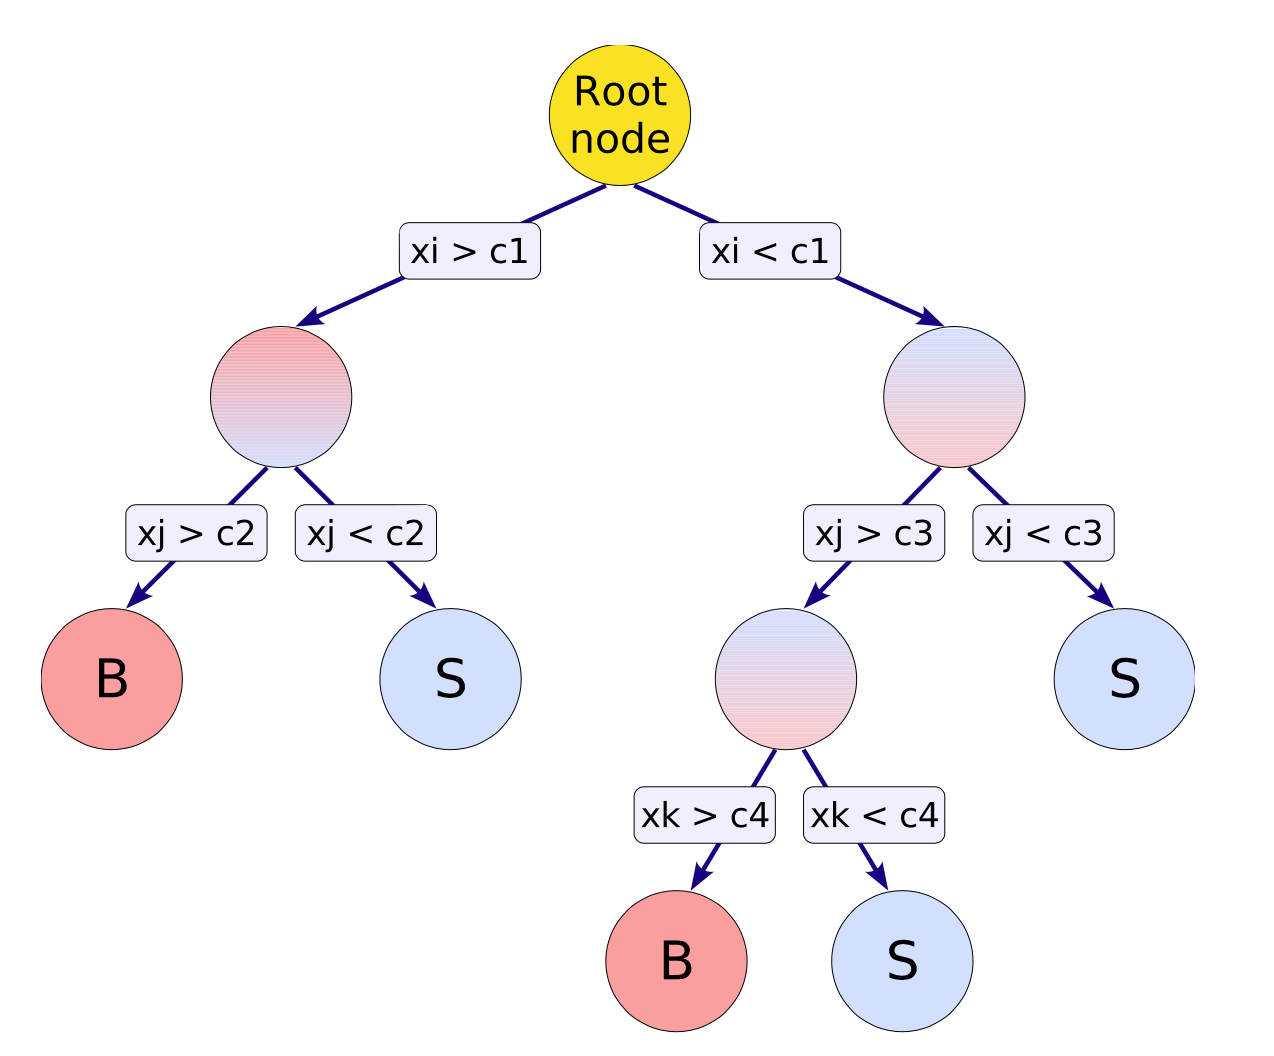
\includegraphics[width=0.5\linewidth]{3_Analysis_techniques/Figures/BDT}
%	\caption{Schematic view of a decision tree. Figure taken from \cite{2007physics3039H}.}
%	\label{fig:BDTexample}
%\end{figure}

% Different trees can be combined into a forest where the final output is determined by the majority vote of all trees, forming the sum of so-called weak learners into one strong learner.   From one training collection, trees are derived by reweighting events, and combined into a single classifier as the  weighted average of each individual decision tree. A method for  making such forests is  boosting a tree. In this method, misclassified events are weighted higher so that future learner concentrate on these events. This has as advantage that the response of the decision trees are stabilised against fluctuations in the training sample which enhances the performance. Additionally, the trees can be kept very shallow, in this thesis the maximal number of nodes is set to three, which improves the robustness against overtraining. Examples of such boosting algorithms are Adaptive Boosting (AdaBoost) and Gradient Boosting~\cite{2014arXiv1403.1452M}. In AdaBoost, each weight of the misclassified events is enhanced while reducing the weight of correctly classified events after each training such that  future events learn those better
%\begin{equation}
% \alpha_{\mathrm{n+1}} = \left(\frac{1-\epsilon_{\mathrm{n}}}{\epsilon_{\mathrm{n}}}\right)^{\beta}, 
%\end{equation}
%where $\epsilon_{\mathrm{n}}$ denotes the misclassification error of the current tree n and $\beta$ is a learning rate. The weight $w_{\mathrm{i}}$ at node i is then equal to $w_{\mathrm{i}} = \mathrm{ln}\:\alpha_{\mathrm{i}}$. The final weight is the sum of all classifiers weighted by their errors. The learning rate is typically chosen to be $\beta\leqslant 0.5$ to allow more boosting steps. Gradient boosting has a similar approach and combines a gradient descent with boosting. Instead of fitting the base-learner to the reweighted data as in AdaBoost, it is fitted to the negative gradient vector of the loss function evaluated at the previous node. Misclassified events will result in a majority vote with large gradients of the loss function. Also for the Gradient boost, the learning rate or shrinkage is typically slow. In this thesis Gradient boost is used with a shrinkage of 0.2-0.3.
%http://www.ccs.neu.edu/home/vip/teach/MLcourse/4_boosting/slides/gradient_boosting.pdf
%https://indico.scc.kit.edu/indico/event/48/session/4/contribution/35/material/slides/0.pdf
%https://arxiv.org/pdf/1403.1452.pdf
%https://www.quora.com/What-is-the-difference-between-gradient-boosting-and-adaboost
% https://people.phys.ethz.ch/~pheno/Lectures2012_StatisticalTools/slides/Chanon2.pdf
%
%Additionally, the Gradient boost is used in combination with bagging, so-called stochastic gradient boosting. Bagging is a resampling technique taking a subset of events  from the training data where the same event is allowed to be randomly picked several times from the parent sample. The tree is then trained on this subset and this is repeated many times. It is based on the assumption that sampling from a dataset that follows a distribution is the same as sampling from the distribution itself~\cite{Behnke:2013:DAH:2564838}. If one draws an event out of the parent sample, it is more likely to draw an event out of the phase space that has a high probability density, as the original dataset will have more events in these regions. Since the selected event is kept in the original sample, the parent sample stays unchanged so that randomly extracted samples have the same parent distribution, albeit statistically fluctuated.  Bagging smears  the statistical fluctuations in the training data, making it suitable for stabilising the response of the classifier and increasing the performance by eliminating overtraining.  In stochastic gradient boosting the bagging resampling procedure uses random sub-samples of the training events for growing the trees. 


The discriminating power of a BDT is assessed by analysing the receiver operating characteristic (ROC) curve. This curve represents the background rejection over the signal efficiency of the remaining sample. The area under the curve (AUC) is compared to  random guessing in order to identify the best classifier can be identified. 
%This follows the Neyman-Pearson lemma that the best ROC curve is given by the likelihood ratio \like(x|Signal)/\like(x|Background)~\cite{Behnke:2013:DAH:2564838}. 
When the multivariate discriminator has no discriminating power, the resulting AUC will be 0\%, while 50\%  means fully separated event classes. In \fig{fig:ROC} examples of ROC curves are shown. 
\begin{figure}[htbp]
	\centering
	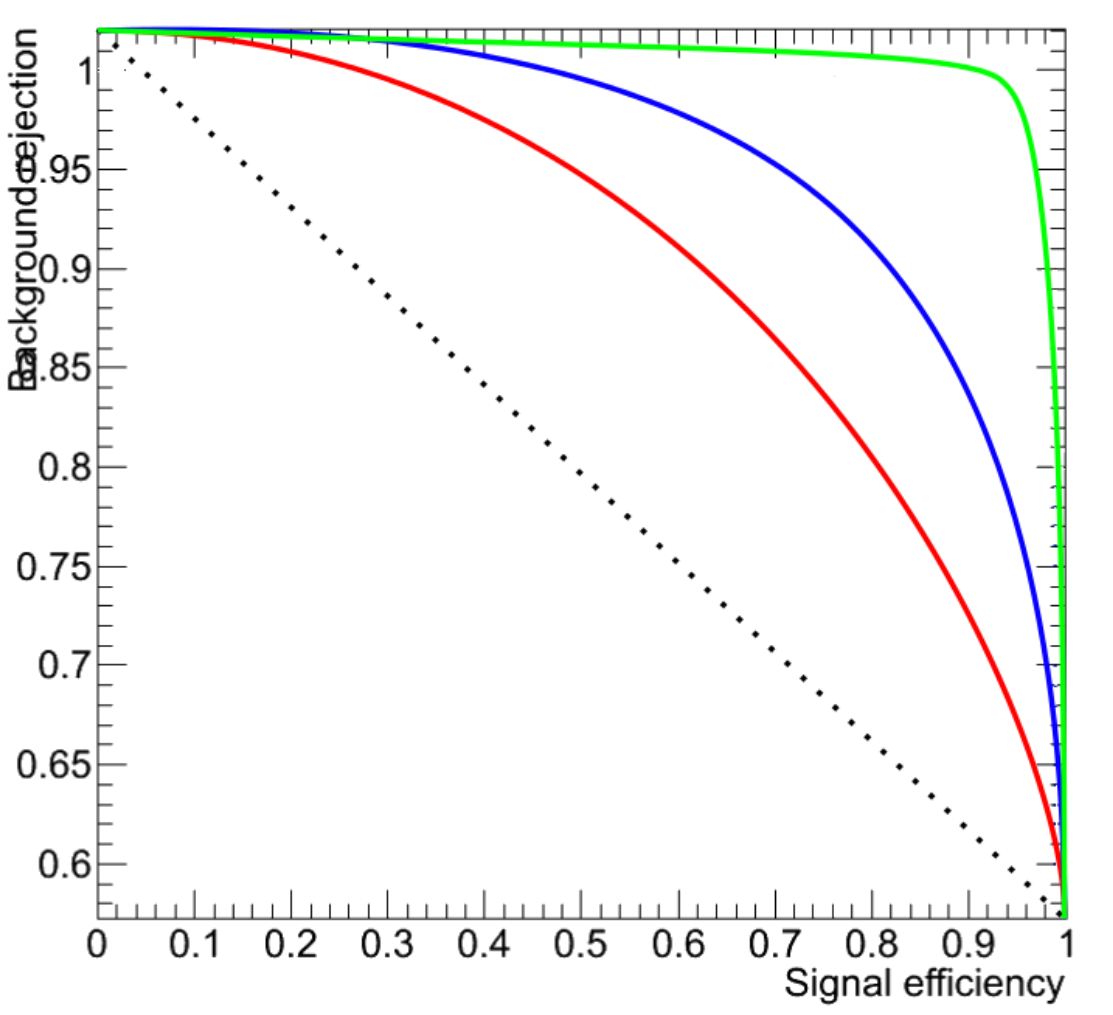
\includegraphics[width=0.7\linewidth]{3_Analysis_techniques/Figures/ROC}
	\caption{Example of ROC curves. In this example, the green method is better than the blue one, which is better than the red one. The dashed line represents a case where there is no separation. Figure taken from \cite{ROC}.}
	\label{fig:ROC}
\end{figure}




\section{Statistical methodology}
\label{sec:Stat}
%VERY GOOD PRESENTATION https://www-conf.slac.stanford.edu/ssi/2012/Presentations/Gross.pdf
%https://arxiv.org/pdf/1503.07622.pdf
The search performed in the framework of this thesis requires the simultaneous analysis of data from different decay channels. The statistical methodology used for this search is developed by the ATLAS and CMS collaborations in the context of the LHC Higgs Combination group~\cite{Chatrchyan:2012tx,Cowan:2010js,CMS-PAS-HIG-12-020,CMS-NOTE-2011-005}. The \texttt{Higgs Combined Tool}~\cite{HiggsCombine} is a 
\texttt{RooStats}~\cite{Moneta:2010pm} framework which runs different statistical methods. In this section, only the statistical tools necessary for the performed search are described~\cite{CLs}.
% The results presented in this thesis are obtained using the asymptotic formulae~\cite{CLs}.

The event yields of signal and background processes are denoted as $s$ and $b$ respectively. These represent event counts in multiple bins or unbinned probability density functions. By use of simulation, predictions on both signal and background yields are made the multiple uncertainties on these predictions are accounted for by introducing nuisance parameters $\theta$ such that $s = s(\theta)$ and $b=b(\theta)$.% In the following, the actual observed events are denoted as data or observation.

%\subsection{The absence of signal: limits}
The Bayesian and modified classical frequentist statistical approaches are used in high energy physics to characterise the absence of a signal.  The level of incompatibility of data with a signal hypothesis is quantified in terms of confidence levels (CL). The convention is to require a 95\% CL for excluding a signal. In general limits are not set on the signal cross section directly, but are set on the signal strength modifier $\mu$. The signal strength modifier is defined such that it equally changes all the cross sections of all production mechanisms of the signal by the same scale.  

%An analysis targeting a certain signal production mechanism can either set approximate model-independent limits on signal cross sections times branching fraction ($\sigma \times \BR$) or on the signal cross section times branching fraction times detector acceptance ($\sigma \times \BR \times \accept$). In order to test various theories, the latter is not useful unless the acceptance \accept\ is provided. However, many analysis are not able to present result in a from of limits  on $\sigma \times \BR (\times \accept)$, therefore an alternative is adopted to set limits in the signal strength modifier $\mu$. The signal strength modifier is defined to equally change all the cross sections of all production mechanisms of the signal by the same scale.  


In this thesis, the modified frequentist approach~\cite{JUNK1999435,0954-3899-28-10-313} for confidence levels that adopts the classical frequentist method to allow nuisance parameters, is used. 
%The classical frequentist  method uses a test statistic $q_{\mu}$ based on the profile likelihood ratio to determine how signal- or background-like the data is. However, it does not allow nuisance parameters and is modified to incorporate these.
Ir constructs a likelihood $\like(\mathrm{data}|\:\mu,\theta)$ is as
\begin{equation}
 \like(\mathrm{data}|\:\mu,\theta) = \mathrm{Poisson}\left(\mathrm{data}|\:\mu s(\theta)+b(\theta)\right) \; \mathrm{pdf}(\tilde{\theta}|\theta).
 \label{eq:like}
\end{equation}
The probability density function $\mathrm{pdf}(\tilde{\theta}|\theta)$ describes all sources of uncertainty. 
In this thesis, all sources of uncertainties are assumed to be either 100\% correlated or uncorrelated. Partially correlated uncertainties are broken down to subcomponents that fit those requirements, allowing to include all constraints in the likelihoods in a clean factorised form. 

A systematic uncertainty pdf $\rho(\theta|\tilde{\theta})$ for the nuisance $\theta$ with nominal value $\tilde{\theta}$ is used.
It reflects the degree of belief of what the true value of the $\theta$ is.  In this thesis, the approach from the \texttt{Higgs Combined Tool} is used where the pdfs $\rho(\theta|\tilde{\theta})$ are re-interpret as posteriors of real or imaginary measurements $\tilde{\theta}$
\begin{equation}
\rho(\theta|\tilde{\theta}) \sim \mathrm{pdf}(\tilde{\theta}|\theta) \: \pi_{\theta}(\theta),
\end{equation}
where $\pi_{\theta}(\theta)$ is the hyper prior for the (imaginary) measurements. The the pdfs used by the \texttt{Higgs Combine Tool} are described in Ref.~\cite{CMS-NOTE-2011-005}. 


The data in \eq{eq:like} represents either the actual observation or pseudo-data to construct sampling distributions. For a binned likelihood, the Poisson probabilities to observe $n_{\mathrm{i}}$ events in bin i is given as
\begin{equation}
 \mathrm{Poisson}\left(\mathrm{data}|\:\mu s(\theta)+b(\theta)\right) = \prod \limits_{\mathrm{i}} \frac{\left(\mu s_{\mathrm{i}}(\theta) + b_{\mathrm{i}}(\theta)\right)^{n_{\mathrm{i}}}}{n_{\mathrm{i}}!} e^{-\mu s_{\mathrm{i}}(\theta)- b_{\mathrm{i}}(\theta)}.
\end{equation}

At the LHC, the test statistic is defined as 
\begin{equation}
q_{\mu} = -2\: \mathrm{ln} \: \frac{\like(\mathrm{data}|\:\mu, \hat{\theta}_{\mu})}{\like(\mathrm{data}|\:\hat{\mu} , \hat{\theta}_{\mu})}, 
\end{equation}
where the likelihood is maximised in the numerator (maximum likelihood estimator, MLE) for a given $\mu$ and (pseudo) data at $\hat{\theta}_{\mu}$, while $\hat{\mu}$ combined with $\hat{\theta}$ defines the point for which the likelihood reaches its global maximum. The estimated signal strength modifier $\hat{\mu}$ can not become negative since a signal rate is positive defined by physics. Furthermore, an upper constraint on the MLE $\hat{\mu} \leq \mu$ is imposed. 
% to guarantee a one sided confidence interval. This has as consequence that upward fluctuations of the data ($\hat{\mu}>\mu$) are not considered against the signal hypothesis of data with a signal with strength $\mu$.  %Note that this definition of the test statistic differs from what has been used at LEP (where “profiling” of systematic errors was not used) and at Tevatron (where systematic errors were profiled, but μ in the denominator was fixed at zero). See Appendix A for details. CMS AN -2011/298

The signal is excluded at $1-\alpha$ confidence level when 
\begin{equation}
\mathrm{CLs} = \frac{\mathrm{P}\left(q_{\mu} \geq q_{\mu}^{\mathrm{obs}}|\: \mu s + b\right)}{\mathrm{P}\left(q_{\mu} \geq q_{\mu}^{\mathrm{obs}}| \:b\right)} \leq \alpha, 
\end{equation}
with $ \mathrm{P}\left(q_{\mu} \geq q_{\mu}^{\mathrm{obs}}|\: \mu s + b\right)$ the probability to observe a value of the test statistic at least as large as the one observed in data $q_{\mu}^{\mathrm{obs}}$, under the signal plus background ($s+b$) hypothesis, and $\mathrm{P}\left(q_{\mu} \geq q_{\mu}^{\mathrm{obs}}|\:  b\right)$ for the background only ($b$) hypothesis. 
These probabilities are defined as 
\begin{equation}
\begin{aligned}
  p_{\mu} &= \mathrm{P}\left(q_{\mu} \geq q_{\mu}^{\mathrm{obs}}|\: \mu s + b\right) = \int \limits_{q^{\mathrm{obs}}_{\mu}}^{\infty} f(q_{\mu}|\: \mu, \hat{\theta}_{\mu}^{\mathrm{obs}}) \:dq_{\mu}, \\
  1-p_{b} &= \mathrm{P}\left(q_{\mu} \geq q_{\mu}^{\mathrm{obs}}|\:  b\right) = \int \limits_{q^{\mathrm{obs}}_{\mu=0}}^{\infty} f(q_{\mu}|\: \mu=0, \hat{\theta}_{\mu=0}^{\mathrm{obs}}) \:dq_{\mu}, 
\end{aligned}
\end{equation}
where $ p_{\mu}$ and $ p_{b}$ are the p-values associated to the two hypothesis, and  $f(q_{\mu}|\: \mu, \hat{\theta}_{\mu}^{\mathrm{obs}})$ and $f(q_{\mu}|\: \mu=0, \hat{\theta}_{\mu=0}^{\mathrm{obs}})$ are the probability density functions of the signal plus background and background only hypothesis constructed from toy Monte Carlo pseudo data. These are generated with nuisance parameters fixed to $\hat{\theta}_{\mu=0}^{\mathrm{obs}}$ (background only) and $\hat{\theta}_{\mu}^{\mathrm{obs}}$ (signal plus backgound).
%These values of the nuisance parameters for the background only $\hat{\theta}_{\mu=0}^{\mathrm{obs}}$ and signal plus background  $\hat{\theta}_{\mu}^{\mathrm{obs}}$ hypothesis that best describe the data are found by maximising the likelihood from \eq{eq:like}. 
%\begin{figure}[htbp]
%	\centering
%	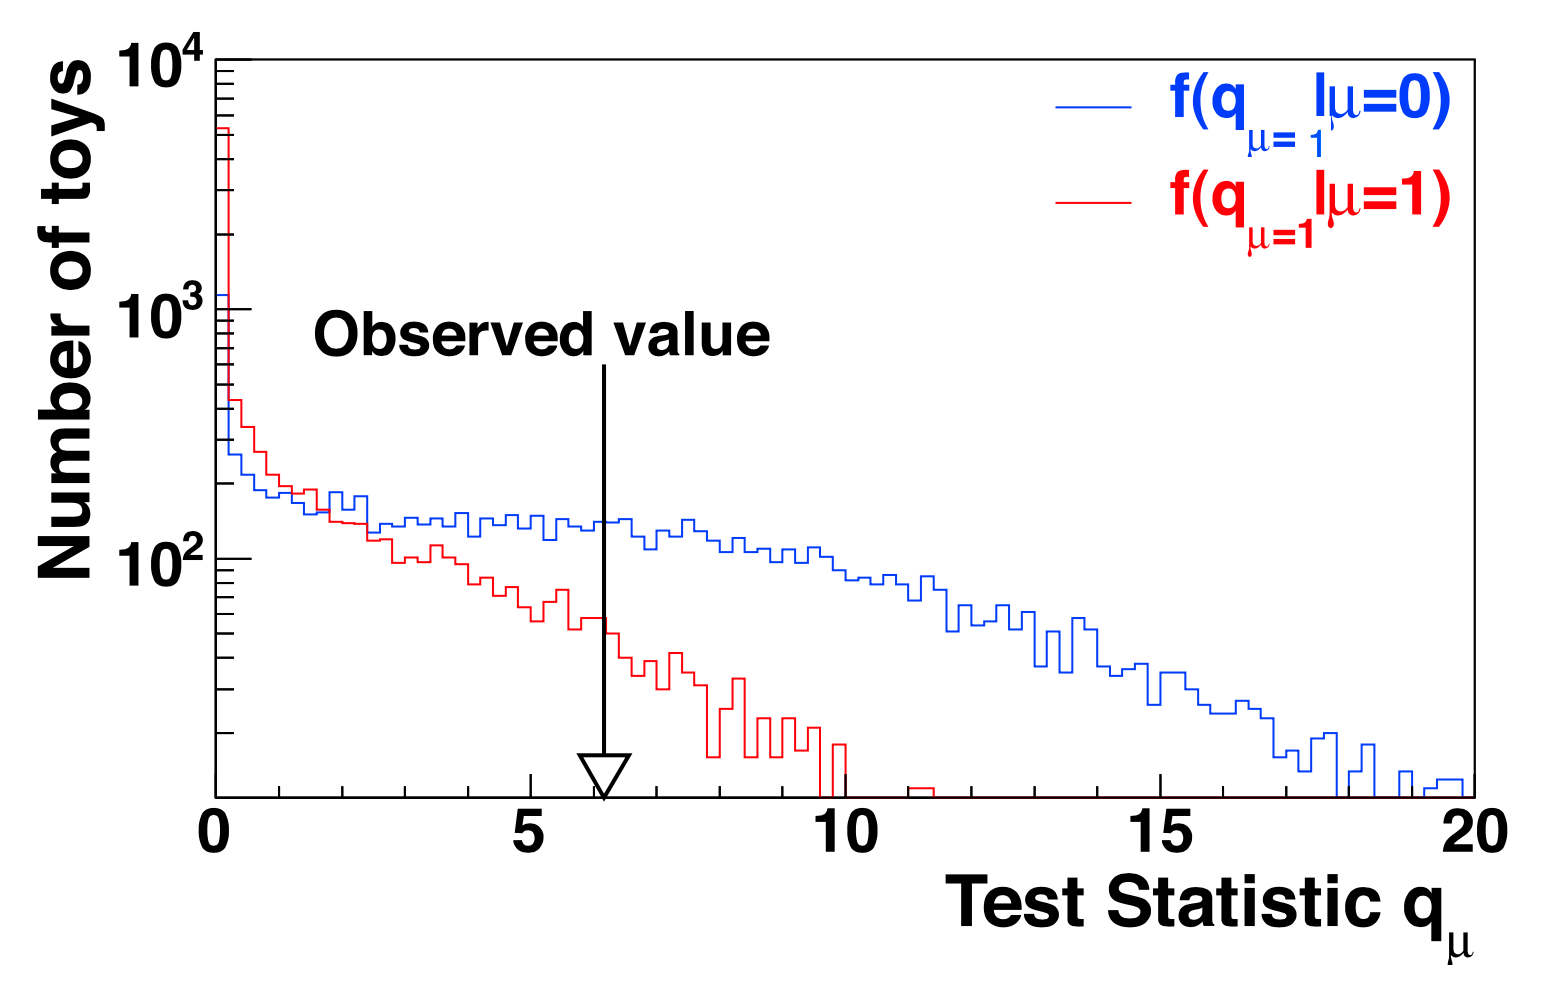
\includegraphics[width=0.7\linewidth]{3_Analysis_techniques/Figures/teststat}
%	\caption{Test statistic distributions for pseudo data generated for the signal plus background ($\mu=1$) and background only ($\mu=0$) hypothesis. Figure taken from \cite{CMS-NOTE-2011-005}.}
%	\label{fig:pdf}
%\end{figure}
\begin{comment}
	Note,
that for the purposes of generating a pseudo-dataset, the nuisance parameters are
fixed to the values θˆobs or θˆobs obtained by fitting the observed data, but are allowed μ0
to float in fits needed to evaluate the test statistic. This way, in which the nuisance parameters are fixed to their maximum likelihood estimates, has good coverage properties [12].
Note that we define pb as pb = P ( q ̃μ < q ̃μ | background-only), excluding the point q ̃μ = q ̃μ . With
these definitions one can identify pμ with CLs+b and pb with 1 − CLb.

If, for μ = 1, CLs ≤ α, we would state that the SM Higgs boson is excluded with (1 − α) CLs confidence level (C.L.). It is known that the CLs method gives conservative limits, i.e. the actual confidence level is higher than (1 − α). See Appendix A for more details.

\end{comment}
The 95\% CL level upper limit on $\mu$ is achieved by adjusting $\mu$ until CL$ = 0.05$, this is the so-called observe limit. The expected median upper limit and the $\pm 1\sigma$ and $\pm 2 \sigma$ bands for a hypothesis is generated by a large set of pseudo data and calculate the CLs and the value of $\mu$ at 95\% CL for each of them. A cumulative probability distribution can be build by starting the integration from the side corresponding to low event yields. The median expected value, so-called expected limit at 95\% CL, is where the cumulative distribution function crosses the 50\% quantile. The $\pm 1 \sigma$ (68\%)  and $\pm 2\sigma$ (95\%) bands on the expected limit are defined by the crossings of the 16\% and 84\%, and 2.5\% and 97.5\% quantiles.
\begin{comment}
	Despite being logically very straightforward, this prescription is not too practical from
126 the computational point of view due to the high CPU demand. If N is the number of
127 “toys” being generated in the internal loop of calculations of the desired quantity and
128 M is a number of pseudo-data sets for which such computation is performed, then the
129 number of times the likelihoods would have to be evaluated in such a linear procedure is
130 N·M.
131 To save on the CPU consumption, we use the fact that the distributions of the test
132 statistic for a given μ do not depend on the pseudo-data, so they can be computed only
133 once. The computation of the p-values for each pseudo-data then requires the test statistic
134 to be evaluated only once for each trial value of μ, and the total number of evaluations is
135 proportionaltoN+MinsteadofN·M.
\end{comment}
%\subsection{Adding sources of uncertainty}
%\label{sec:Nuis}
%\begin{comment}
% IN frequentist mehod wordt er geen unc op data beschouwd. Je hebt 1 chocolade bar of je hebt het niet. De enige onz komt van of je 1 chocolade bar verwachtte
%\end{comment}
%In this thesis, all sources of uncertainties are assumed to be either 100\% correlated or uncorrelated. Partially correlated uncertainties are broken down to subcomponents that fit those requirements, allowing to include all constraints in the likelihoods in a clean factorised form. 
%
% A systematic uncertainty pdf $\rho(\theta|\tilde{\theta})$ for the nuisance $\theta$ with nominal value $\tilde{\theta}$ is used.
% It reflects the degree of belief of what the true value of the $\theta$ is.  In this thesis, the approach from the \texttt{Higgs Combined Tool} is used where the pdfs $\rho(\theta|\tilde{\theta})$ are re-interpret as posteriors of real or imaginary measurements $\tilde{\theta}$
% \begin{equation}
% 	\rho(\theta|\tilde{\theta}) \sim p(\tilde{\theta}|\theta) \: \pi_{\theta}(\theta),
% \end{equation}
% where $\pi_{\theta}(\theta)$ is the hyper prior for the (imaginary) measurements. For the pdfs used by the \texttt{Higgs Combine Tool} (normal, log normal, gamma distribution), hyper priors can remain flat. This allows to use the pdf $p(\tilde{\theta}|\theta)$ to constrain the likelihood of the main measurement in a frequentist calculation. Additionally this allows to build a sampling distribution of the test statistic~\cite{CMS-NOTE-2011-005}. 
% 
% The statistical uncertainties on the Monte Carlo prediction in each bin are obtained following the  Barlow-Beeston-light approach~\cite{Conway:2011in}. In this approach a single Gaussian constrained nuisance parameter is assigned to scale the sum of the process yields in each bin, constrained by the total uncertainty. This method has as advantage that it minimises the number of parameters required in the maximum likelihood fit.
% Considering $n_{\mathrm{tot}}$ events in a bin with background processes i in the bin
% \begin{equation}
% n_{\mathrm{tot}} = \sum \limits_{\mathrm{i} \:\in \:\mathrm{bkg}} n_{\mathrm{i}},
% \end{equation}
% the total uncertainty $e_{\mathrm{tot}}$ is given by 
% \begin{equation}
% e_{\mathrm{tot}} = \sqrt{ \sum \limits_{\mathrm{i}\: \in\: \mathrm{bkg}} e_{\mathrm{i}}^2}, 
% \end{equation}
% with $ e_{\mathrm{i}}$ the uncertainty on background i and is given by the sum of  squares of weights used to fill the bins. The Gaussian constrained parameter $x$ has then a nominal value of zero and scales the yield as $n_{\mathrm{tot}}+x\:e_{\mathrm{tot}}$. 
% %https://indico.cern.ch/event/107747/contributions/32677/attachments/24367/35056/Conway-PhyStat2011.pdf
% %http://w3.iihe.ac.be/~pvanlaer/RooStats/statistics_2012_part3_v9.pdf
 
%\subsubsection*{Choices of systematic uncertainty density functions}
%For uncertainties that are unconstrained by a priori measurements that do not involve the data going into the statistical analysis, flat priors are used. When there are a priori measurements available such as those from control regions, one can use either a Gaussian pdf,  a log-normal pdf, or a  gamma distribution. The Gaussian pdf is suited for describing uncertainties on parameters with both positive and negative values. This prior is however not suitable for positively defined observables such as cross sections, cut efficiencies, luminosity, etc. and is not used in this thesis. An alternative option is the log normal pdf which is used in the rest of this thesis
%\begin{equation}
%  \rho(\theta|\tilde{\theta}) = \frac{1}{\sqrt{2\pi} \:\mathrm{ln}\;(\kappa)} \mathrm{exp}\left(-\frac{(\mathrm{ln}\:(\theta/\tilde{\theta}))^2}{2 (\mathrm{ln}\: \kappa)^2}\right) \frac{1}{\theta}. 
%\end{equation}
%The parameter $\kappa$ characterises the width of the log normal pdf. For example $\kappa = 1.10$ implies that the observable can be larger or smaller by a factor 1.10, both deviation having a chance of 16\%. The gamma distribution is used for describing statistical uncertainties associated with a number of Monte Carlo events in simulation or a number of observed events in a data control sample. In this thesis, the gamma distribution is only used for the latter. The event rate in the signal region $n$ is related to the number of events in the control region $N$ as $n= \alpha N$. Ignoring the uncertainties on $\alpha$, the predicted rate follows 
%\begin{equation}
%	\rho(n|N) = \frac{1}{\alpha} \frac{n/\alpha)^N}{N!} \mathrm{exp}(-n/\alpha). 
%\end{equation}
%The mapping between the posteriors $\rho(\theta|\tilde{\theta})$ and the auxiliary measurement pdfs $p(\tilde{\theta}|\theta)$ are given in \cite{CMS-NOTE-2011-005}.

%The \texttt{Higgs Combined Tool} allows the overall expected rate of a particular process to float and include a Gaussian constraint on them. 

%\subsection{Asymptotic approximation of the CL method}
%\label{sec:NuisAsym}
In order to significantly reduce computing time, the Asymptotic CL method is used. This method  avoids an ensemble of toy Monte Carlo samples and instead replaces it by one representative dataset, called Asimov dataset. This dataset is constructed such that all observed quantities are set equal to their MLE values ($\hat{\theta}_{\mathrm{Asimov}}= \theta_0$). More information about this procedure can be found in Refs. \cite{Cowan:2010js}.
%https://indico.cern.ch/event/74940/contributions/2088584/attachments/1047729/1493442/Wald-Asimov.pdf
%\subsection{Extracting the signal model parameters}
%From a scan of the profile likelihood ratio, 
%\begin{equation}
%q(\mu) = -2\: \mathrm{ln} \: \frac{\like(\mathrm{obs}|\:s(/mu) + b, \hat{\theta}_{\mu})}{\like(\mathrm{obs}|\:s(\hat{\mu})  + b, \hat{\theta})}, 
%\end{equation}
%the signal model parameters are evaluated.  The likelihood is maximised by the parameters $\hat{\mu}$ and $\hat{\theta}$. The likelihood 
%\begin{equation}
% \like_{\mathrm{max}} = \like(\mathrm{obs}|\:s(\hat{\mu}) + b, \hat{\theta})
%\end{equation}
%is called the best-fit set. 
%
%The 68\% and 95\% CL on a given parameter of interest $\mu_{\mathrm{i}}$ is then evaluated from $q(\mu_{\mathrm{i}}) = 1$ or $q(\mu_{\mathrm{i}}) = 3.84$ respectively, where all other unconstrained model parameters are treated in the same way as the nuisance parameters~\cite{CMS-PAS-HIG-12-020}. 
%


%http://cds.cern.ch/record/1460438/files/HIG-12-020-pas.pdf
%\subsection{Confidence levels }

%https://indico.cern.ch/event/614672/timetable/#20170907
